\documentclass[11pt]{article}
\usepackage{comment}
\usepackage{graphicx}
\usepackage{fourier-orns}
\usepackage{algorithm, algpseudocode}
\usepackage{tabto}
\usepackage{amsmath, amsthm, amssymb, amsfonts}
\usepackage{color}
\usepackage{fancyhdr}
\usepackage{enumitem}
\usepackage{latexsym}
\usepackage{multicol}
\usepackage{tikz}
\usetikzlibrary{arrows}
\usepackage{url}
\topmargin=-.5in
\textheight=9.0in
\evensidemargin=0in
\oddsidemargin=0.0in
\textwidth=6.5in

\title{CS182 Homework \# 05}
\author{Maninder (Kaurman) Kaur}

\begin{document}

\maketitle

\section*{Question 0}
\begin{quote}
    \textit{I, Maninder (Kaurman) Kaur, affirm that I have not given or received any unauthorized help on this assignment and that this work is my own. What I have submitted is expressed and explained in my own words. I have not used any online websites that provide a solution. I will not post any parts of this problem set to any online platform and doing so is a violation of course policy.}
\end{quote}

\clearpage
\section*{Question 1}

    \textbf{A multinational company uses six character strings to identify each employee, where the only characters used are $\{1,2,3,4,5,A,B,C,D,E\}$. No characters are repeated.}
    \begin{enumerate}[label=(\alph*)]
        \item How many codes begin and end with a letter?
        \item How many codes contain exactly 3 digits, and they appear consecutively as a block in the code?
        \item How many codes have no two letters adjacent?
        \item If all valid employee identification codes are listed in lexicographic ordering $1 < 2 < \cdots < 4 < 5 < A < B < \cdots < D < E$, what is the rank (position) of the code C3A1B2 in a dictionary of these codes?
    \end{enumerate}

    \subsection*{Solution}
    \begin{enumerate}[label=(\alph*)]
        \item
        \begin{itemize}
            \item[] Total of 6 positions, index 1 and 6 must be letters, while index 2-5 can be either. \\
            Index 1 and 6: \(P(5,2) = 5 \cdot 4 = 20\) \\
            Index 2-5: \(P(8,4)= 8 \cdot7\cdot6\cdot5=1680\) \\
            \textbf{Answer:} \(20 \cdot 1680\) codes
        \end{itemize}
        \item
        \begin{itemize}
            \item[] From the wording of the problem, there has to be exactly 3 digits and exactly 3 letters, and where the digits are put together. \\
            Possible places for the digit block: Positions 1-3, 2-4, 3-5, and 4-6. \\
            \# of ways for digits and numbers to be\(\binom{5}{3} \cdot 3! = 10 \cdot 6 = 60\) \\
            \(4 \cdot 60 \cdot 60\) \(\rightarrow\) 4 starting positions for the digits, 60 combinations for the 3 digits, 60 combinations for the 3 letters. \\
            \textbf{Answer:} 14400 codes \\
        \end{itemize}
        \item
        \begin{itemize}
            \item[] There are 6 total positions in the code, no char repetition. Only the 5 letters cannot be adjacent (next to). Suppose there exists a letter \(n\) that is \(6 > n\) and represents how many letters there are in a code. \\
            \(6-n\) meaning there are \(\binom{5}{6-n}\) ways to choose letters from 5 of the ltter choices. \\
            Since there are 5 possible digits \(6-n \leq 5, k \geq1\) \\
            There are also 5 letters so \(k \leq 5\)
            From the amount of gaps we can have: \(n \leq 7-n\) so \(k \leq \lfloor \frac{7}{2} \rfloor = 3\). Meaning n can equal 1,2, or 3. \\ \\
            If \(n = 1\): \(\binom{5}{1} \cdot \binom{5}{5} \cdot \binom{6}{1} \cdot 1! \cdot 5! = 3600\) \\ \\
            If \(n = 2\): \(\binom{5}{2} \cdot \binom{5}{4} \cdot \binom{5}{2} \cdot 2! \cdot 4! = 12000\) \\ \\
            If \(n = 3\): \(\binom{5}{3} \cdot \binom{5}{3} \cdot \binom{4}{3} \cdot 3! \cdot 3! = 14400\) \\ \\
            \(3600+12000+14400\) \\ \\
            \textbf{Answer:} 30000 codes
        \end{itemize}
        \item
        \begin{itemize}
            \item[] Each index of the code has a either a letter or number that holds some lexicographic position. To find the rank of each position, you need to find 1 + the number of codes that come before the indeces. We need to use permutations to count lexicographically smaller by each index left to right. \\
            \((P(9,5) \cdot 7) + (P(8,4) \cdot 2) + (P(7,3) \cdot 4) + (P(5,1) \cdot 3) + 0\) \\ \\
            \textbf{Answer:} Rank 110056
        \end{itemize}
    \end{enumerate}

\clearpage
\section*{Question 2}

    \textbf{A new robotics club BoilerBots is formed by students in the CS department and the Mechanical Engineering department. The CS students consist of 5 freshmen, 3 sophomores, 2 juniors (Rakesh and Dave), and 2 seniors (Alice and Bob). The Mechanical Engineering students consist of 6 freshmen, 12 sophomores, 4 juniors, and 2 seniors.}
    \begin{enumerate}[label=(\alph*)]
        \item The BoilerBots needs to organize a visit from 5 of the CS student members to do outreach at the local elementary school. How many ways can we organize this visit such that exactly 2 freshmen, 1 sophomore, 1 junior, and 1 senior take part?
        \item We need to form a 5 member CS advisory committee from the 12 CS student members subject to the following constraints: (i) Alice and Bob refuse to serve together. (ii) Rakesh insists that Dave joins any committee that Rakesh joins. Count the number of ways such a committee can be formed.
        \item All 36 students of the BoilerBots club must decide on the order to list their names on the website. The arrangement must satisfy the following conditions: (a) Each of the freshmen must be immediately preceded by one of the sophomores. (b) The juniors refuse to be listed next to one another.
    \end{enumerate}

    \subsection*{Solution}
    \begin{enumerate}[label=(\alph*)]
        \item
        \begin{itemize}
            \item[] \(\binom{5}{2} \cdot \binom{3}{1} \cdot \binom{2}{1} \cdot \binom{2}{1}\) \\ 
            \(10 \cdot 3 \cdot 2 \cdot 2\)
            \textbf{Answer:} 120 ways
        \end{itemize}
        \item
        \begin{itemize}
            \item[] Total ways, no constraints: \(\binom{12}{5} = \frac{12 \cdot 11 \cdot10 \cdot9 \cdot 8}{5 \cdot4 \cdot3 \cdot2 \cdot1} = 792\) \\ \\
        \(|A|\) = Commitee w/o Alice and Bob \(\binom{10}{3} = \frac{10 \cdot9 \cdot8}{3 \cdot2 \cdot1} = 120\) \\ \\
        \(|B|\) = Comitee w/Rakesh w/o Dave \(\binom{10}{4} = \frac{10 \cdot9 \cdot8 \cdot7}{4 \cdot3 \cdot2 \cdot1} = 210\) \\ \\
        \(A \cap B = \binom{9}{2} = \frac{9 \cdot8}{2 \cdot 1} = 36\) \\ \\ 
        \(A \cup B = 120 + 210 -36 = 294\) \\ 
        792 - 294 \\
        \textbf{Answer:} 498 ways 
        \end{itemize}
        \item
        \begin{itemize}
            \item[] 

% Handling the freshman-sophomore pair condition
Pair $11$ freshmen with $11$ sophomores:
\(
\binom{15}{11} \cdot 11!
\) 

% Ensuring no two juniors are adjacent
Choose $6$ positions with at least one gap between them:
\(
\binom{25 - 6 + 1}{6} = \binom{20}{6}
\) 

Arrange $6$ juniors:
\(
6!
\)

% Arranging remaining units
Arrange $19$ remaining positions:
\(
19!
\)

\(
\binom{15}{11} \cdot 11! \cdot \binom{20}{6} \cdot 6! \cdot 19!
\)

% Final answer
\textbf{Answer}:
\(
1365 \cdot 11! \cdot 38760 \cdot 6! \cdot 19!
\)

            
        \end{itemize}
    \end{enumerate}

\clearpage
\section*{Question 3}

    \textbf{Alice flips a fair coin repeatedly and notes down each flip by using "H" to indicate heads and "T" to indicate tails. For example, HH refers to a heads followed by a heads and TH refers to a tails followed by a heads.}
    \begin{enumerate}[label=(\alph*)]
        \item What is the probability that the 3rd heads occurs on the 10th flip? Assume that she stops flipping once the 3rd heads has occurred.
        \item What is the probability that she sees "HHT" before "HTH"?
    \end{enumerate}

    \subsection*{Solution}
    \begin{enumerate}[label=(\alph*)]
        \item
        \begin{itemize}
            \item[] In the first 9 flips, we need to have 2 heads, and there needs tro be 7 tails with 2 heads in total of 9 flips. \\ \\
            \(\binom{9}{2} \cdot \binom{1}{2}^9 \cdot \frac{1}{2}\) \\ \\
            \textbf{Answer:} \(\frac{9}{256}\)
        \end{itemize}
        \item
        \begin{itemize}
            \item[] Define states based on the longest suffix that matches a prefix of ``HHT'' or ``HTH'':
\begin{itemize}
    \item[] \( S \): Start (no progress).
    \item[] \( H \): Ends in H.
    \item[] \( HH \): Ends in HH.
    \item[] \( HT \): Ends in HT.
    \item[] \( HHT \): Reached HHT (absorbing, success).
    \item[] \( HTH \): Reached HTH (absorbing, failure).
\end{itemize}


Let \( P_s \) be the probability of reaching HHT before HTH from state \( s \).
\begin{itemize}
    \item [] Absorbing states: \( P_{HHT} = 1 \), \( P_{HTH} = 0 \).
    \item[] Equations
    \(
    P_S = \frac{1}{2} P_H + \frac{1}{2} P_S \implies \frac{1}{2} P_S = \frac{1}{2} P_H \implies P_S = P_H
    \)
    \(
    P_H = \frac{1}{2} P_{HH} + \frac{1}{2} P_{HT}
    \)
    \(
    P_{HH} = \frac{1}{2} P_{HH} + \frac{1}{2} P_{HHT} = \frac{1}{2} P_{HH} + \frac{1}{2} \implies \frac{1}{2} P_{HH} = \frac{1}{2} \implies P_{HH} = 1
    \)
    \(
    P_{HT} = \frac{1}{2} P_{HTH} + \frac{1}{2} P_S = \frac{1}{2} \cdot 0 + \frac{1}{2} P_S = \frac{1}{2} P_S
    \)
    \item [] Substitute:
    \(
    P_H = \frac{1}{2} \cdot 1 + \frac{1}{2} \cdot \frac{1}{2} P_S = \frac{1}{2} + \frac{1}{4} P_S
    \)
    Since \( P_S = P_H \):
    \(
    P_S = \frac{1}{2} + \frac{1}{4} P_S \implies P_S - \frac{1}{4} P_S = \frac{1}{2} \implies \frac{3}{4} P_S = \frac{1}{2} \implies P_S = \frac{\frac{1}{2}}{\frac{3}{4}} = \frac{2}{3}
    \)
\end{itemize}

\textbf{Answer}: \( \frac{2}{3} \)
        \end{itemize}
    \end{enumerate}


\clearpage
\section*{Question 4}

    \textbf{In a rural village, 1\% of the wells are contaminated with EColi. Contaminated wells produce cloudy water 80\% of the time, while clean wells still run cloudy 5\% of the time. If a well's water is cloudy, the health department runs a coliform test. If the water is cloudy and contaminated, the test returns positive 98\% of the time and the test returns positive 8\% of the time given that the water is cloudy but clean (free of contamination). If we draw a sample of water from a well that returns a positive coliform test and the water is cloudy, find the probability that the sample is actually contaminated.}
    \begin{enumerate}[label=(\alph*)]
        \item[] \textbf{Note:} $P(A \cap B | C) = P(A | B \cap C)P(B | C)$. This is the multiplication rule in conditional probability.
    \end{enumerate}

    \subsection*{Solution}
    \begin{enumerate}[label=(\alph*)]
        \item []
        \begin{itemize}
            \item[] We need to find \(P(C| W \cap T)\) or the probability that the well is contaminated given there is cloudy water AND a positive test. \\ \\
            \(P(C| W \cap T) = \frac{(P(T| W \cap C)P(W|C))P(C)}{P(W \cap T)}\) \\ \\
            \(P(C| W \cap T) = \frac{P(W \cap T | C)P(C)}{P(W \cap T)}\) \\ \\
            \(P(C| W \cap T) = \frac{P(W \cap T | C)P(C)}{P(W \cap T) = P(W \cap T | C) P(C) + P(W \cap T | C^c) P(C^c)}\) \\ \\
            \(P(C| W \cap T) = \frac{(0.784 \cdot 0.01)}{(0.00784 + 0.00396)}\) \\ \\
            \(P(C| W \cap T) = \frac{784}{1180}\) \\ \\
            \textbf{Answer:} \(\frac{196}{295}\)
        \end{itemize}
    \end{enumerate}


\clearpage
\section*{Question 5}

    \textbf{A submarine is missing. You believe that it was equally likely to have gone down in any of 5 possible regions. If the submarine is in region $i$, then the probability that the submarine will be found is $1 - \beta_i$ ($i=1,2,3,4,5$) for some $0 < \beta_i < 1$. We call $\beta_i$ as an "overlook probability" because it means the probability of failing to find the submarine in region $i$ during a search, given that it is actually located in region $i$. For each $i=1,2,3,4,5$, calculate the conditional probability that the submarine is in the $i$th region given that a search of region 3 was unsuccessful.}
    \begin{enumerate}[label=(\alph*)]
        \item[] 
    \end{enumerate}

    \subsection*{Solution}
    \begin{enumerate}[label=(\alph*)]
        \item []
        \begin{itemize}
            \item[]  
            % Defining the problem
Let \( S_i \) denote the event that the submarine is in region \( i \) (\( i=1,2,3,4,5 \)), with \( P(S_i) = \frac{1}{5} \). \\
Let \( F_3 \) denote the event that a search of region 3 is unsuccessful \\
Compute \( P(S_i | F_3) \) for each \( i = 1, 2, 3, 4, 5 \) \\

% Applying Bayes' Theorem

\(
P(S_i | F_3) = \frac{P(F_3 | S_i) P(S_i)}{P(F_3)}
\) \\


% Numerator
For \( i = 3 \): \( P(F_3 | S_3) P(S_3) = \beta_3 \cdot \frac{1}{5} \)\\
For \( i = 1, 2, 4, 5 \): \( P(F_3 | S_i) P(S_i) = 1 \cdot \frac{1}{5} = \frac{1}{5} \) \\

% Denominator: Total probability of F_3
\(
P(F_3) = \sum_{i=1}^5 P(F_3 | S_i) P(S_i)
\) \\
\(
= P(F_3 | S_1) P(S_1) + P(F_3 | S_2) P(S_2) + P(F_3 | S_3) P(S_3) + P(F_3 | S_4) P(S_4) + P(F_3 | S_5) P(S_5)
\) \\
\(
= 1 \cdot \frac{1}{5} + 1 \cdot \frac{1}{5} + \beta_3 \cdot \frac{1}{5} + 1 \cdot \frac{1}{5} + 1 \cdot \frac{1}{5} = \frac{1 + 1 + \beta_3 + 1 + 1}{5} = \frac{4 + \beta_3}{5}
\) \\

% Conditional probabilities
- For \( i = 1 \):
\(
P(S_1 | F_3) = \frac{P(F_3 | S_1) P(S_1)}{P(F_3)} = \frac{1 \cdot \frac{1}{5}}{\frac{4 + \beta_3}{5}} = \frac{\frac{1}{5}}{\frac{4 + \beta_3}{5}} = \frac{1}{4 + \beta_3}
\) \\
- For \( i = 2 \):
\(
P(S_2 | F_3) = \frac{1 \cdot \frac{1}{5}}{\frac{4 + \beta_3}{5}} = \frac{1}{4 + \beta_3}
\) \\
- For \( i = 3 \):
\(
P(S_3 | F_3) = \frac{\beta_3 \cdot \frac{1}{5}}{\frac{4 + \beta_3}{5}} = \frac{\beta_3}{4 + \beta_3}
\) \\
- For \( i = 4 \):
\(
P(S_4 | F_3) = \frac{1 \cdot \frac{1}{5}}{\frac{4 + \beta_3}{5}} = \frac{1}{4 + \beta_3}
\) \\
- For \( i = 5 \):
\(
P(S_5 | F_3) = \frac{1 \cdot \frac{1}{5}}{\frac{4 + \beta_3}{5}} = \frac{1}{4 + \beta_3}
\) \\

% Verification
Sum of probabilities:
\(
\frac{1 + 1 + \beta_3 + 1 + 1}{4 + \beta_3} = \frac{4 + \beta_3}{4 + \beta_3} = 1
\) \\
        \end{itemize}
    \end{enumerate}


\clearpage
\section*{Question 6}

    \begin{enumerate}[label=(\alph*)]
        \item List an Eulerian path of the graph.
        \item List a Hamiltonian path of the graph.
        \item The graph currently has neither an Eulerian circuit nor a Hamiltonian circuit. How many more edges do you need to add to make the graph both Eulerian circuit and Hamiltonian circuit? Specify the edge(s) and explain briefly.
    \end{enumerate}

    \subsection*{Solution}
    \begin{enumerate}[label=(\alph*)]
        \item
        \begin{itemize}
            \item[] Eularian paty is a path that goes through each edge once. We will go between these vertexes to get to each all the edges:
            \((vA,vD) \rightarrow(vD, vE) \rightarrow (vE,vA) \rightarrow(vA,vB) \rightarrow (vB,vF) \rightarrow(vF,vD) \rightarrow(vD,vC), \rightarrow (vC,vB) \rightarrow (vvB,vG) \rightarrow (vG.vF)\)
        \end{itemize}
        \item
        \begin{itemize}
            \item[] Hamiltonian path is a path that visits every vertex once. We will go to these vertexes: \(A \rightarrow E \rightarrow D \rightarrow C \rightarrow B \rightarrow G \rightarrow F\)
        \end{itemize}
        \item
        \begin{itemize}
            \item[]  An edge between between A and F. For Hamiltonian, from the above, it will be able to return to A. With Eularian, it is the same thing from part A, where the edge finishes at the starting vertex edge. 
        \end{itemize}
    \end{enumerate}

    \clearpage
\section*{Question 7}

    \textbf{Consider a graph $G$ with the vertex set $V=\{v_1, v_2, v_3, v_4, v_5, v_6\}$ and the edge set $E=\{(v_1, v_2), (v_2, v_3), (v_3, v_4), (v_4, v_5), (v_5, v_1), (v_1, v_3), (v_4, v_6)\}$.}
    \begin{enumerate}[label=(\alph*)]
        \item Draw the graph $G$.
        \item Determine the chromatic number $\chi(G)$ of the graph.
        \item What is the minimum number of edge(s) you need to remove from $G$ to make the graph bipartite? List the edge(s) you need to remove and provide the two vertex sets (each partition) of the resulting bipartite graph.
    \end{enumerate}

    \subsection*{Solution}
    \begin{enumerate}[label=(\alph*)]
        \item
        \begin{itemize}
            \item[] 

                \begin{figure}[htbp] % [htbp] are placement options (here, top, bottom, page)
        \centering % Centers the image horizontally
        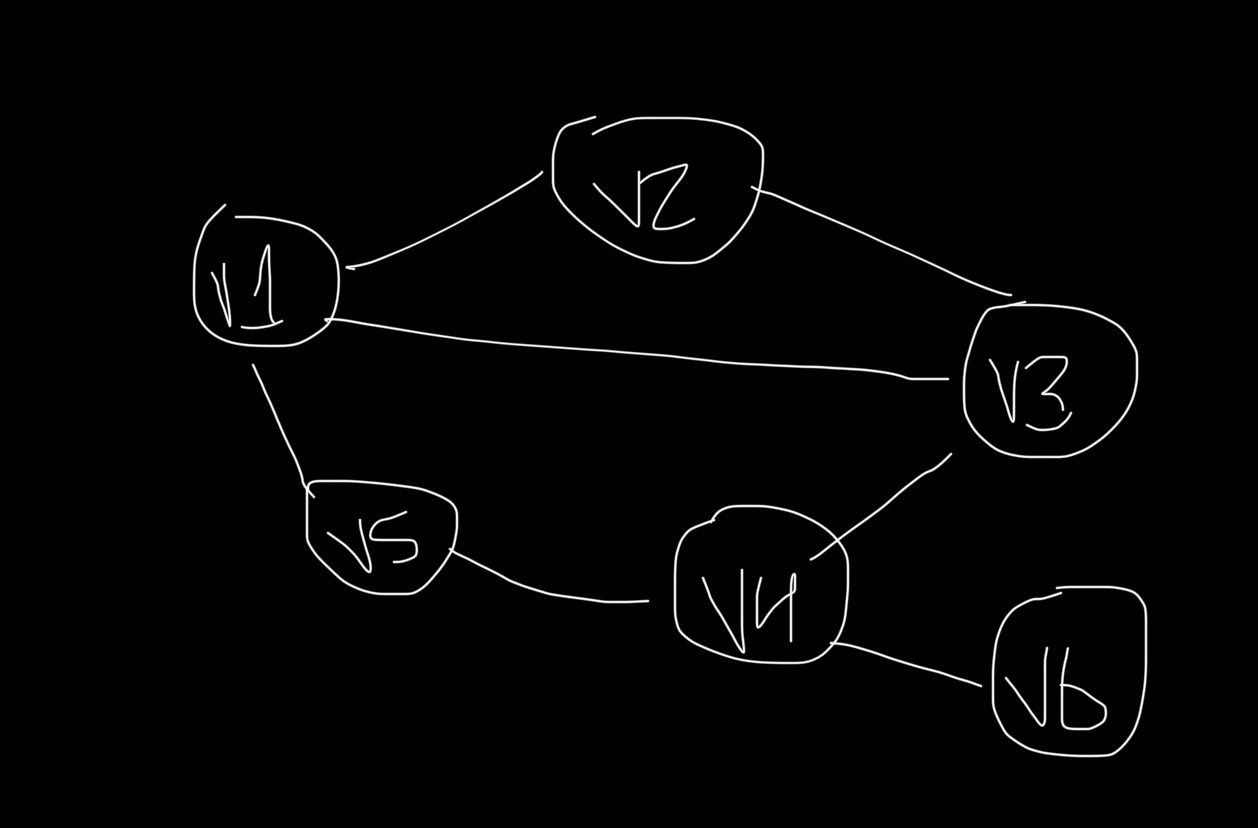
\includegraphics[width=0.5\linewidth]{cs182/IMG_2199.jpeg} % Include the image
        \label{fig:your_image_label} % Label for cross-referencing
                \end{figure}
            
        \end{itemize}
        \item
        \begin{itemize}
            \item[] 
                \begin{figure}[htbp] % [htbp] are placement options (here, top, bottom, page)
        \centering % Centers the image horizontally
        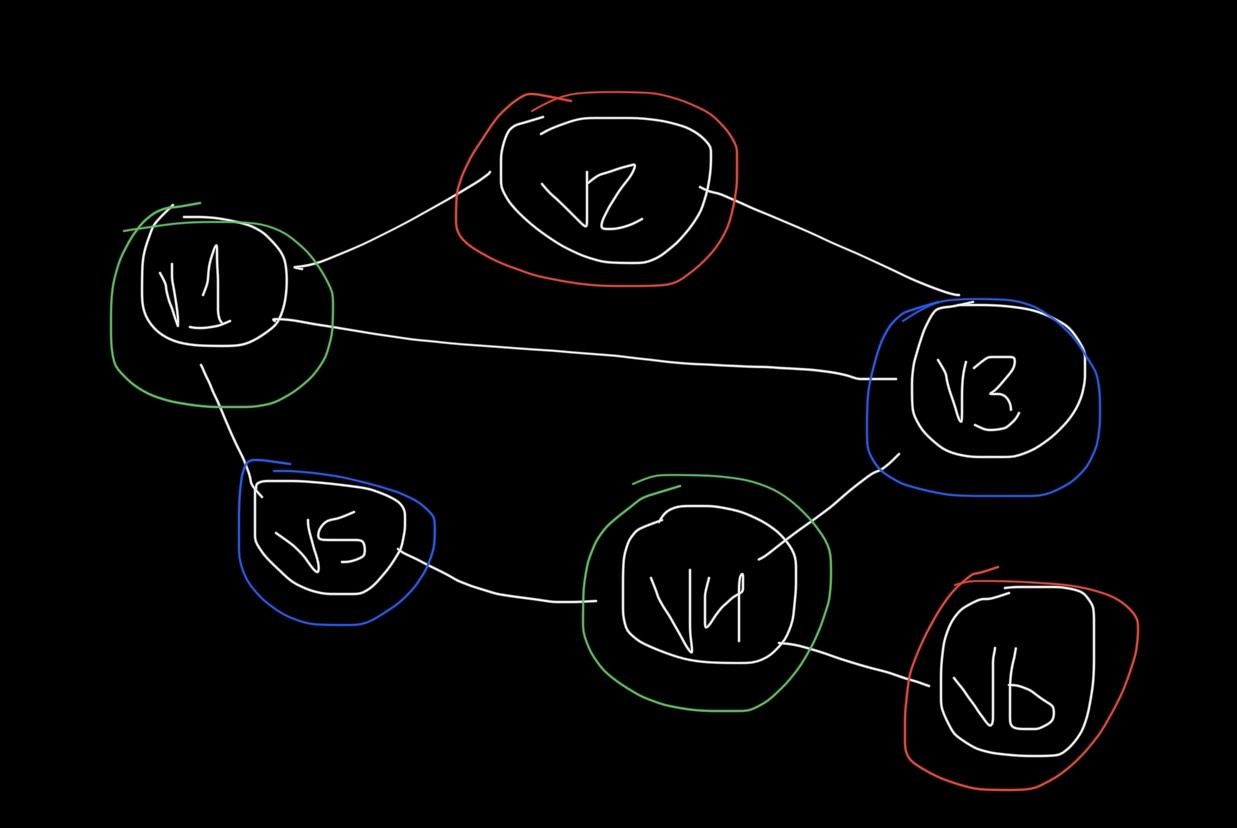
\includegraphics[width=0.5\linewidth]{cs182/IMG_2200.jpeg} % Include the image
        \label{fig:your_image_label} % Label for cross-referencing
                \end{figure}
            
            \textbf{Answer:} $\chi(G) = 3$  \\ \\
        \end{itemize}
        \item
        \begin{itemize}
            \item[] 

% Test removing one edge
Remove \( (v_2, v_3) \): \\
Edges left: \( (v_1, v_2), (v_3, v_4), (v_4, v_5), (v_5, v_1), (v_1, v_3), (v_4, v_6) \) \\
5-cycle broken (no \( v_2-v_3 \)) \\
Triangle broken (no \( v_2-v_3 \)) \\
Remaining graph: Paths \( v_1-v_5-v_4-v_3 \), \( v_1-v_2 \), edge \( v_4-v_6 \) \\
Partitions: \( X = \{v_1, v_4\} \), \( Y = \{v_2, v_3, v_5, v_6\} \) \\
Edges \( (v_1, v_2), (v_1, v_5), (v_1, v_3), (v_3, v_4), (v_4, v_5), (v_4, v_6) \) are between \( X \) and \( Y \) \\

% Final answer
\textbf{Answer: }
\(
\text{(c) } 1 \text{ edge } (v_2, v_3), \text{ partitions } \{v_1, v_4\}, \{v_2, v_3, v_5, v_6\}
\)

        \end{itemize}
    \end{enumerate}


\clearpage
\section*{Question 8}

    \textbf{You are the manager of Purdue's networking system. You received a report about the details on the network's 75 servers and their direct, two-way connections. The report claims that the server consists of the following: Firewall: 17 servers, each connected to exactly 3 other servers. Database Servers: 30 servers, each connected to exactly 8 other servers. Application servers: 28 servers, each connected to exactly $k$ other servers. Later, you got a new report with the fixed configuration. The corrected report states that there are 18 Firewall servers and 27 application servers (Database server remained the same). In the corrected network, the total number of connections is exactly 242.}
    \begin{enumerate}[label=(\alph*)]
        \item You think the report is flawed. Prove that this network configuration is impossible. Justify your answer using the handshake theorem.
        \item Later, you got a new report with the fixed configuration. The corrected report states
that there are 18 Firewall servers and 27 application servers (Database server remained
the same). In the corrected network, the total number of connection is exactly 282.
Find the degree $k$.
    \end{enumerate}

    \subsection*{Solution}
    \begin{enumerate}[label=(\alph*)]
        \item
        \begin{itemize}
            \item[] % Defining the problem parameters
\(\sum \text{deg}(v) = 2E\).

% Calculating the sum of degrees
Firewall servers: \( 17 \cdot 3 = 51 \) \\
Database servers: \( 30 \cdot 8 = 240 \) \\
Application servers: \( 28 \cdot k = 28k \) \\

% Applying the Handshake Theorem
Total sum of degrees:
\(
51 + 240 + 28k = 291 + 28k
\)
by the Handshake Theorem, \(291 + 28k\) must be even, as it equals \( 2E \), where \( E \) is the number of edges (an integer). \\ \\
The sum \( 291 + 28k \) is odd (odd + even = odd), which cannot equal \( 2E \) (which is even). This is a contradiction, as the sum of degrees must be even. \\
\textbf{Answer:} Impossible
        \end{itemize}
        \item
        \begin{itemize}
            \item[]


Firewall servers: \( 18 \cdot 3 = 54 \) \\
Database servers: \( 30 \cdot 8 = 240 \) \\
Application servers: \( 27 \cdot k = 27k \) \\

Total sum of degrees:
\(
54 + 240 + 27k = 294 + 27k
\) \\
By the Handshake Theorem:
\(
294 + 27k = 2 \cdot 282 = 564
\) \\
Solve for \( k \):
\(
294 + 27k = 564
\) \\
\(
27k = 564 - 294 = 270
\) \\
\(
k = \frac{270}{27} = 10
\) \\
% Verifying the solution
The sum of degrees is:
\(
294 + 27 \cdot 10 = 294 + 270 = 564
\) \\
\textbf{Answer:} k = 10
        \end{itemize}
    \end{enumerate}





\end{document}
